\documentclass{beamer}
\usepackage[spanish]{babel}
\usepackage[latin1]{inputenc}
\usepackage{multicol} % indice en 2 columnas
\usepackage{centernot}
\usepackage{amsmath}% http://ctan.org/pkg/amsmath

\usepackage{color}


\usepackage{graphicx}
\graphicspath{ {im/} }


\newcommand{\notimplies}{%
  \mathrel{{\ooalign{\hidewidth$\not\phantom{=}$\hidewidth\cr$\implies$}}}}


\usetheme{Warsaw}
%\usecolortheme{crane}
\useoutertheme{shadow}
\useinnertheme{rectangles}

\setbeamertemplate{navigation symbols}{} % quitar simbolitos


\title[Tema 6 - Programaci\'on Lineal]{Programaci\'on lineal}
\subtitle{Estudios de Ingenier\'ia}
\author[https://frogames.es]{
Juan Gabriel Gomila%$^{1}$  \and E. Eva$^{2}$ \and S. Serpiente$^{3}$
}
\institute[Frogames]{
 % $^{1-2}$
 Frogames
   \and
  \texttt{https://frogames.es}
}
\date{\today}

\AtBeginSection{
\begin{frame}
  \begin{multicols}{2}
  \tableofcontents[currentsection]   
\end{multicols}
\end{frame}
}

\AtBeginSubsection{
\begin{frame}
  \begin{multicols}{2}
  \tableofcontents[currentsection,currentsubsection]
\end{multicols}
\end{frame}
}



%empieza aqui


\begin{document} 

\frame{\titlepage}

\begin{frame}
  \frametitle{\'Indice}
  \tableofcontents
\end{frame}

\section{Introducci\'on}

\begin{frame}
\frametitle{Introducci\'on}
Se comenzar\'a el tema mostrando diversos ejemplos que se pueden modelizar mediante t\'ecnicas de programaci\'on lineal.

El objetivo de la programaci\'on lineal es optimizar (minimizar o maximizar) una funci\'on lineal de $n$ variables sujetas a restricciones de igualdad o desigualdad, tambi\'en lineales.
\end{frame}


\begin{frame}
\frametitle{Introducci\'on}
La programaci\'on lineal se aplica en diversos campos, como por ejemplo:
\begin{itemize}
\item Log\'istica: problema del transporte.
\item Mezclas: problema de la dieta.
\item Finanzas.
\item Mercadotecnia.
\item Asignaci\'on de tareas. 
\item Producci\'on.
\item Otras decisiones.
\end{itemize}
\end{frame}

\begin{frame}
\frametitle{Introducci\'on}
Cualquier problema de programaci\'on lineal requiere cuatro componentes b\'asicos:
\begin{enumerate}
\item El conjunto de datos del problema.
\item El conjunto de variables que intervienen en el problema, junto con sus dominios de definici\'on.
\item El conjunto de restricciones del problema que definen el conjunto de soluciones admisibles.
\item La funci\'on que se ha de optimizar.
\end{enumerate}
\end{frame}


\begin{frame}
\frametitle{El problema del transporte}
El problema del transporte se refiere al proceso de determinar el n\'umero de mercanc\'ias que se han de llevar desde cada uno de los or\'igenes a cada uno de los destino posibles.

El objetivo suele ser minimizar el coste del transporte y las restricciones vienen dadas por las capacidades de producci\'on de cada origen y las necesidades de cada destinaci\'on.

\end{frame}


\begin{frame}
\frametitle{El problema del transporte}
\begin{figure}[h]
\label{fig:volumen}
\centering
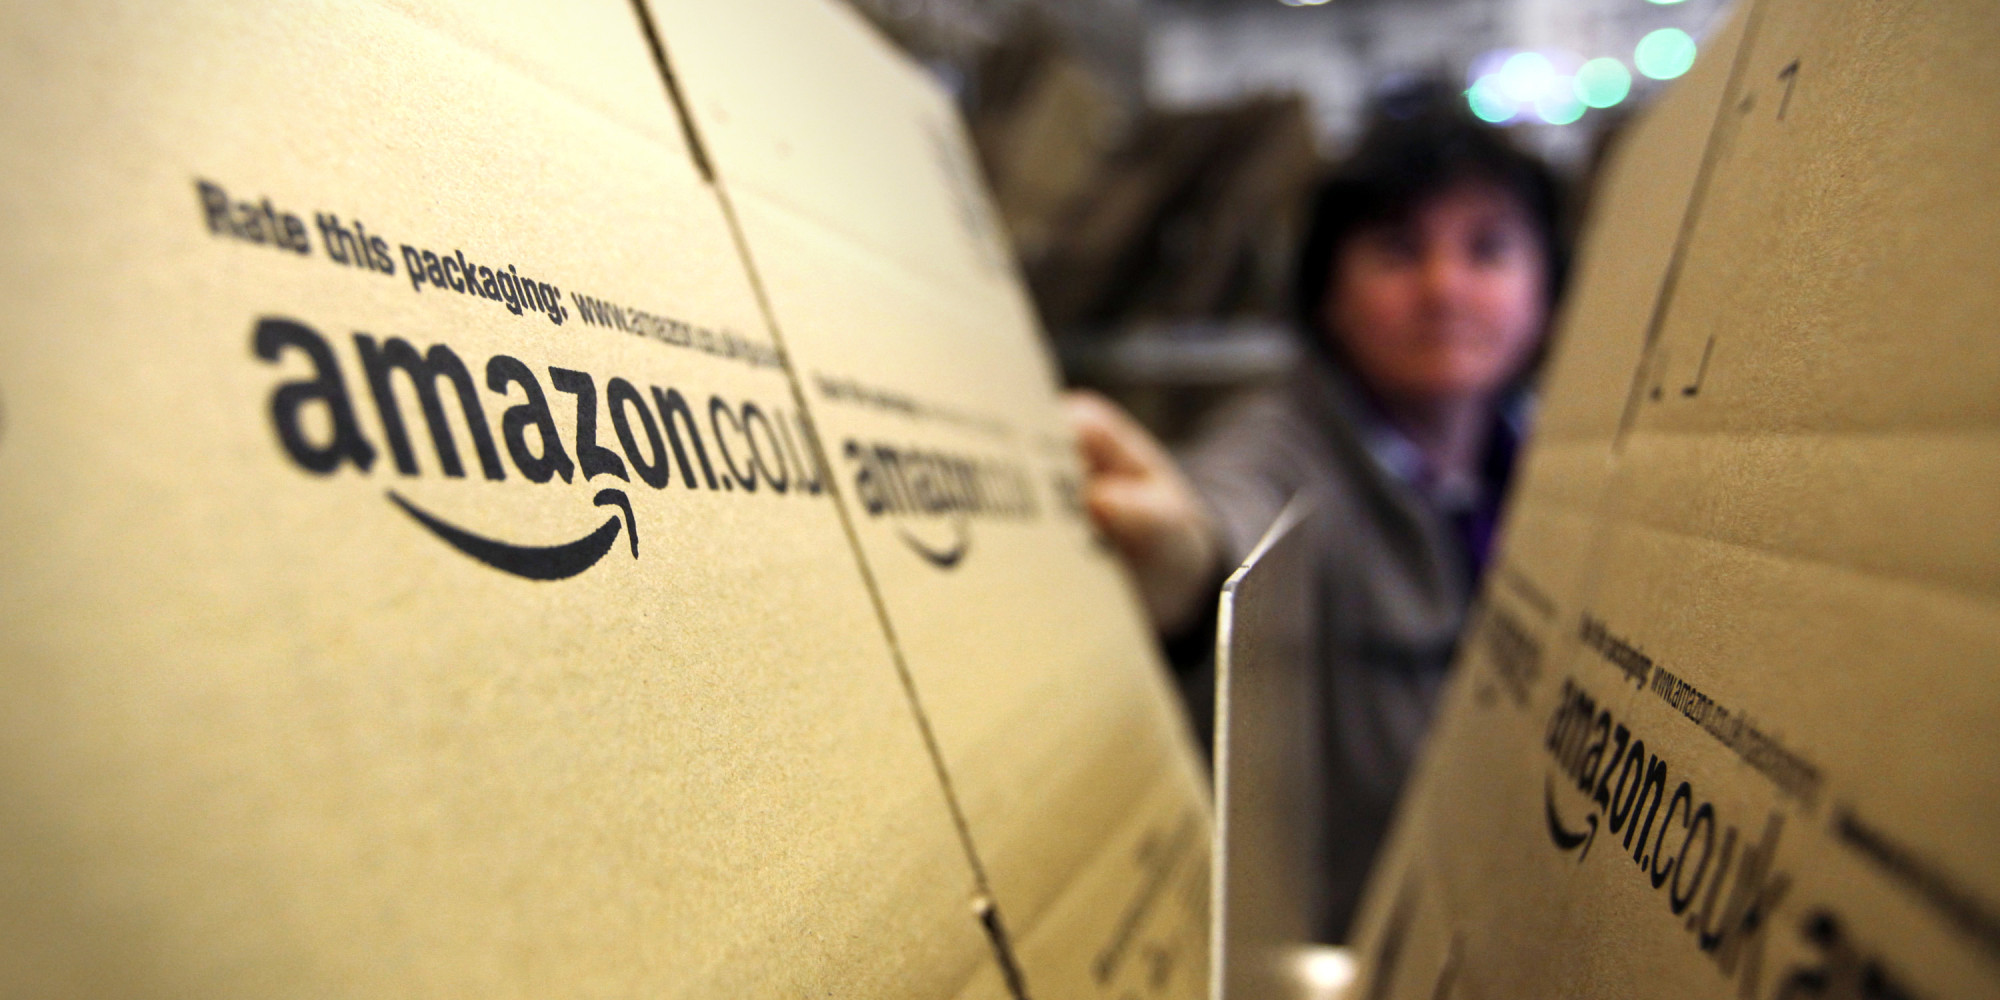
\includegraphics[width=\textwidth]{amazon}
\end{figure}
\end{frame}

\begin{frame}
\frametitle{El problema del transporte}
Sup\'ongase que un determinado producto se ha de llevar en cantidades $u_1, u_2, \cdots, u_m$ desde $m$ puntos de origen y se ha de recibir en $n$ destinos en cantidades $v_1, v_2, \cdots, v_n$.

El problema consiste en determinar las cantidades $x_{ij}$ que se han de llevar desde el origen $i$ al destino $j$ para minimizar el coste del transporte.

Los cuatros elementos principales del problema son:
\end{frame}

\begin{frame}
\frametitle{El problema del transporte}
\begin{itemize}
\item[1] Datos:
\begin{itemize}
\item $m$: n\'umero de or\'igenes.
\item $n$: n\'umero de destinos.
\item $u_i$: cantidad de producto que se ha de llevar desde el origen $i$
\item $v_j$: cantidad de producto que se ha de recibir en el destino $j$
\item $c_{ij}$: coste de llevar una unidad de producto desde $i$ hasta $j$
\end{itemize}
\end{itemize}
\end{frame}

\begin{frame}
\frametitle{El problema del transporte}
\begin{itemize}
\item[2] Variables:
\begin{itemize}
\item $x_{ij}$: cantidad de producto que se lleva desde $i$ hasta $j$, con $x_{ij}\geq 0$ para todo $i=1,\cdots,m$ y para todo $j=1\cdots, n$ (dominio de definici\'on de las variables)
\end{itemize}
\end{itemize}
\end{frame}


\begin{frame}
\frametitle{El problema del transporte}
\begin{itemize}
\item[3] Restricciones:
\begin{itemize}
\item La cantidad total del producto que surge de $i$ ($u_i$) ha de coincidir con la suma de las cantidades que surgen de $i$ a cada destino $j=1,\cdots, n$:
\[\sum_{j=1}^n x_{ij} = u_i \]
\item La cantidad total de producto que recibe $j$ ($v_i$) ha de coincidir con la suma de cantidades que lleguen a $j$ desde todos los or\'igenes $i=1,\cdots, m$:
\[\sum_{i=1}^m x_{ij} = v_j \]
\end{itemize}
\end{itemize}
\end{frame}

\begin{frame}
\frametitle{El problema del transporte}
\begin{itemize}
\item[4] Objetivo:

En este caso, se va a minimizar el coste del env\'io.
\end{itemize}
\end{frame}


\begin{frame}
\frametitle{El problema del transporte}
\begin{figure}[h]
\label{fig:volumen}
\centering
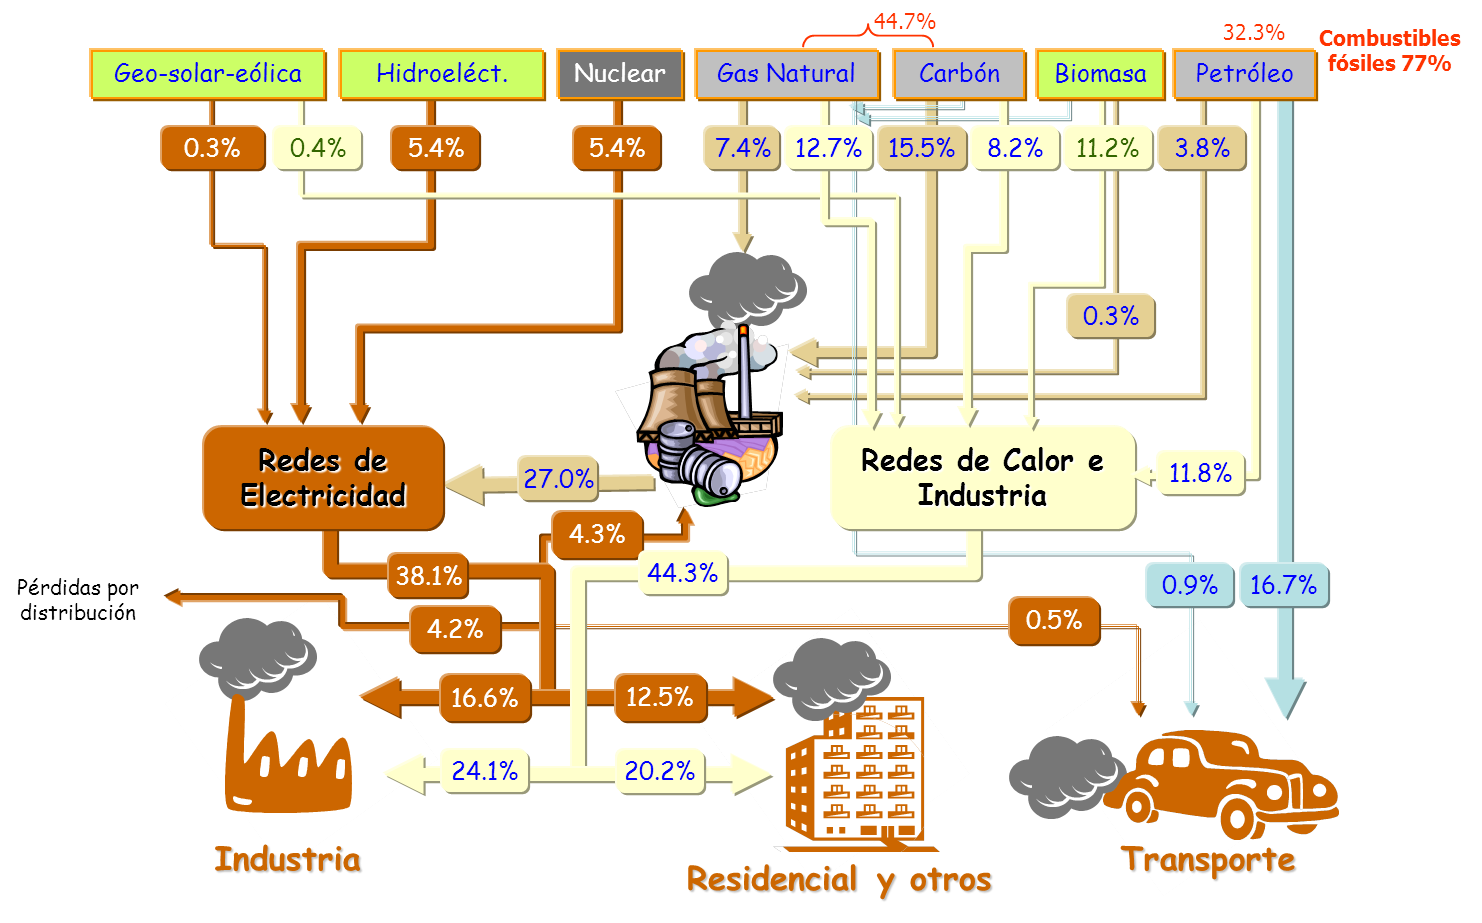
\includegraphics[width=\textwidth]{problema_transporte}
\end{figure}
\end{frame}


\begin{frame}
\frametitle{El problema del transporte - Ejemplo}
Una compa\~n\'ia de \'ambito nacional produce y distribuye  una l\'inea de neveras de alta eficiencia energ\'etica. La empresa tiene l\'ineas de producci\'on y montaje en dos ciudades, Pamplona y Bilbao, y tres cadenas de distribuci\'on localizadas en Madrid, Barcelona y Sevilla.

La oficina de Madrid presenta una demanda anual de 10000 neveras, la de Sevilla 8000 y la de Barcelona 15000.

La planta de Bilbao puede producir hasta 20.000 neveras anuales y la de Pamplona 15000. 

Los costes de transporte por unidad (en euros) son los siguientes:

\begin{tabular}{ |p{2.5cm}||p{2.3cm}|p{2.3cm}|p{2.3cm}|  }
 \hline
 \multicolumn{4}{|c|}{Costes de transporte por unidad (en euros)} \\
 \hline
 Origen/Destino& Madrid &Barcelona&Sevilla\\
 \hline
 Pamplona   & 3    &1&   5\\
 Bilbao &   2  & 2   &4\\
 \hline
\end{tabular}
Se plantea un problema de programaci\'on lineal que minimiza los costes anuales de la compa\~n\'ia.
\end{frame}

\begin{frame}
\frametitle{Mezclas. El problema de la dieta}
El problema de la dieta representa una de las primeras aplicaciones de la programaci\'on lineal que se utiliza en hospitales. Se usa para determinar la dieta de los pacientes que satisfaciendo unas especificaciones nutritivas m\'inimas de la forma m\'as barata posible.

Actualmente tambi\'en se aplica en el sector de la ganader\'ia con la misma idea; encontrar la combinaci\'on \'optima de alimentos que consiguen una aportaci\'on nutritiva m\'inima suponiendo el menor coste posible. Una aplicaci\'on de este problema se muestra en el siguiente ejemplo:
\end{frame}


\begin{frame}
\frametitle{Mezclas. El problema de la dieta - Ejemplo}
Un ganadero se quiere asegurar de que sus animales ingieren diariamente al menos 14 unidades de hierro, doce de vitamina A y 18 de vitamina C.

Un kilogramo de harina tiene un coste de dos euros y cuenta con una unidad de hierro, una de vitamina A y tres de vitamina C. Un kilogramo de ma\'iz tiene un coste de dos euros y contiene dos unidades de hierro, una de vitamina A y una de vitamina C.
Determ\'inense las posibles maneras de alimentar al ganado que satisfagan las necesidades m\'inimas alimenticias diarias con el m\'inimo coste posible.
\end{frame}



\begin{frame}
\frametitle{Producci\'on - Ejemplo}
Una empresa fabrica cuatro tipos de corbata. Una de seda, otra de poli\'ester y dos de poli\'ester y algod\'on. La tabla siguiente muestra el coste en euros de los materiales y de su disponibilidad:
\begin{tabular}{ |p{2.5cm}||p{2.8cm}|p{4cm}|  }
 \hline
 \multicolumn{3}{|c|}{Costes y disponibilidad de los materiales} \\
 \hline
 Material & Coste por metro & Metros disponibles/mes\\
 \hline
 Seda   & 21    &800\\
 Poli\'ester &   6  & 3000\\
 Algod\'on &   9  & 1600\\
 \hline
\end{tabular}
\end{frame}

\begin{frame}
\frametitle{Producci\'on - Ejemplos}
La tabla siguiente muestra todos los datos relativos a la producci\'on, la demanda mensual y la composici\'on de cada tipo de corbata:
\begin{tabular}{ |p{1.5cm}||p{1.8cm}|p{2.4cm}|p{1.6cm}|p{2cm}|  }
 \hline
 \multicolumn{5}{|c|}{Propiedades} \\
 \hline
 Tipos& Prendas vendidas &Demanda min/max & Metros necesarios & Composici\'on\\
 \hline
 Seda   & 6.70    &6000 - 7000 &  0.125 & 100\% seda\\
 Poliester   & 3.55    &10000 - 14000 &  0.08 & 100\% pol\\
 Pol/Alg   & 4.31    &13000 - 16000 &  0.10 & 50\%pol - 50\%cot�\\
 Pol/Alg   & 4.81    &6000 - 8500 &  0.1. & 30\%pol - 70\%cot�\\
 \hline
\end{tabular}
Plant\'eese un problema de programaci\'on lineal para determinar el plan de producci\'on que maximiza los beneficios de la empresa.
\end{frame}


\begin{frame}
\frametitle{Planificaci\'on de horarios}
La planificaci\'on de horarios intenta dar respuesta efectiva a las necesidades de personal durante un periodo de tiempo concreto.

Sectores t\'ipicos donde se hace esta programaci\'on lineal para tomar decisiones sobre la planificaci\'on de horarios son las entidades bancarias y los grandes almacenes.
\end{frame}


\begin{frame}
\frametitle{Planificaci\'on de horarios- Ejemplos}
Sup\'ongase que una entidad bancaria necesita diariamente entre 10 y 18 cajeros en funci\'on de la hora del d\'ia. Las necesidades diarias se especifican en la tabla siguiente:
\begin{tabular}{ |p{4cm}||p{4cm}|  }
 \hline
 \multicolumn{2}{|c|}{Disponibilidad} \\
 \hline
 Franja horaria& Num. Cajeros\\
 \hline
 9a.m. - 10a.m.   & 10\\
 10a.m. - 11a.m.   & 12\\
 11a.m. - 12a.m.   & 14\\
 12a.m. - 1p.m.   & 16\\
 1p.m. - 2p.m.   & 18\\
 2p.m. - 3p.m.   & 17\\
 3p.m. - 4p.m.   & 15\\
 4p.m. - 5p.m.   & 10\\

 \hline
\end{tabular}
\end{frame}


\begin{frame}
\frametitle{Planificaci\'on de horarios- Ejemplos}
La oficina tiene 12 trabajadores a jornada completa y dispone de personal suficiente para trabajar a media jornada. Un cajero que trabaja a media jornada debe estar operativo 4 horas al d\'ia y estar disponible para comenzar a trabajar a cualquier hora entre las nueve de la ma\~nana y la una de la tarde. Los trabajadores a jornada completa deben estar operativos desde las nueve de la ma\~nana hasta las cinco de la tarde y tienen una hora libre para comer (la mitad come de once a doce y la otra mitad lo hace de doce a una).

Las normas de la entidad limitan el n\'umero de horas realizadas por los trabajadores a tiempo parcial a, como mucho, el 50\% de las horas diarias que se realicen. (N\'otese que se realizan 112 horas diarias). Estos trabajadores ganan 16 euros al d\'ia y los trabajadores a jornada completa 50 euros al d\'ia.

Se plantea un problema de programaci\'on lineal que establece un horario que minimiza los costes salariales del banco.
\end{frame}


\begin{frame}
\frametitle{Finanzas. Selecci\'on de una cartera de valores - Ejemplos}
Un banco invierte en cr\'edito al consumo, bonos corporativos, dep\'ositos de oro y pr\'estamos a la construcci.\'on. Actualmente dispone de cinco millones de euros para invertir y pretende, por un lado maximizar el inter\'es esperado para los pr\'oximos seis meses y por el otro cumplir con la diversificaci\'on propugnada por la Junta Directiva seg\'un se especifica en la tabla siguiente:

\begin{tabular}{ |p{3.3cm}||p{3cm}|p{3cm}|  }
 \hline
 \multicolumn{3}{|c|}{Finanzas} \\
 \hline
 Tipos de inversi\'on& Inter\'es esperado &L\'imite de inversi\'on (millones de euros)\\
 \hline
 Cr\'editos al consumo   & 7\%    &1\\
 Bonos corporativos   & 11\%    &2.5\\
 Dep\'ositos de oro   & 19\%    &1.5\\
 Pr\'estamos constr. & 15\%    &1.8\\
    \hline
\end{tabular}

\end{frame}


\begin{frame}
\frametitle{Finanzas. Selecci\'on de una cartera de valores - Ejemplos}

La Directiva tambi\'en exige que como m\'inimo un 55\% de los fondos se dediquen a dep\'ositos de oro y pr\'estamos a la construcci\'on, mientras que el porcentaje dedicado a los cr\'editos al consumidor no han de superar el 15\% de los fondos.

Se plantea un problema de programaci\'on lineal que optimice el objetivo del banco.
\end{frame}


\begin{frame}
\frametitle{Mercadotecnia}


La programaci\'on lineal se utiliza en el campo de la mercadotecnia y la publicidad como una herramienta que permite determinar cu\'al es la combinaci\'on m\'as efectiva de medios para anunciar los productos de una empresa.

Muchas veces la empresa dispone de un presupuesto fijo para publicidad y el objetivo es distribuir este presupuesto entre diversas opciones (TV, radio, diarios, revistas, Google, Facebook...) de manera que los productos de una empresa tengan la m\'axima difusi\'on. En otros casos, las restricciones vienen dadas por la disponibilidad de medios y de las pol\'iticas publicitarias de la empresa. Se ver\'a una aplicaci\'on con el siguiente ejemplo:
\end{frame}



\begin{frame}
\frametitle{Mercadotecnia - Ejemplo}
Una cadena nacional de locales de ocio dispone de 8000 euros semanales para publicidad. Este dinero se ha de destinar a publicar anuncios en TV, diarios y dos emisoras de radio.

El objetivo final es conseguir la mayor audiencia posible.

La tabla siguiente recoge toda la informaci\'on referente a la audiencia esperada por anuncio, el coste (en euros) de cada anuncio y el n\'umero m\'aximo de anuncios semanales posibles en cada medio.

\begin{tabular}{ |p{2cm}||p{2cm}|p{2cm}|p{2.8cm}|  }
 \hline
 \multicolumn{4}{|c|}{Mercadotecnia} \\
 \hline
 Medio& Audiencia &Coste & N\'umero m\'aximo\\
 \hline
 TV   & 5000   &800&12\\
 Diario & 8500 &925&5\\
 Radio 1   & 2400  &290&25\\
 Radio 2  & 2800   &380&20\\
    \hline
\end{tabular}
\end{frame}




\begin{frame}
\frametitle{Mercadotecnia - Ejemplo}
La empresa tambi\'en exige la contrataci\'on de un m\'inimo de 5 anuncios por radio semanales y no se puede destinar a este medio m\'as de 1800 euros por semana.
Plant\'eese un problema de programaci\'on lineal que optimice el objetivo de la empresa.
\end{frame}




\begin{frame}
\frametitle{Investigaci\'on de mercados}
 La programaci\'on lineal tambi\'en se aplica al estudio de mercados. Mediante el siguiente ejemplo se puede ver como las estad\'isticas pueden emplear la programaci\'on lineal para el dise\~no de encuestas.
 \end{frame}




\begin{frame}
\frametitle{Investigaci\'on de mercados - Ejemplo}
Se va a realizar una encuesta para determianar la opini\'on de los ciudadanos de Baleares sobre la inmigraci\'on. La encuesta ha de satisfacer lo siguiente:
\begin{enumerate}
\item Entrevistar un m\'inimo de 2300 familias baleares.
\item En al menos 1000 familias entrevistadas, la persona de m\'as edad no debe superar los 30 a\~nos.
\item En al menos 600 familias entrevistadas, la edad de la persona mayor ha de estar comprendida entre los 31 y los 50 a\~nos.
\item El porcentaje de familias entrevistadas que pertenecen a zonas con alta tasa de inmigraci\'on no ha de ser inferior al 15\% del total.
\end{enumerate}
Todas las encuentas se han de hacer personalmente y ha de responder la persona m\'as mayor de cada familia.
\end{frame}




\begin{frame}
\frametitle{Investigaci\'on de mercados - Ejemplo}
La tabla siguiente indica el coste (en euros) de cada encuesta seg\'un la edad del encuestado y si pertenece o no a una zona con tasa elevada de inmigraci\'on.

\begin{tabular}{ |p{3cm}||p{2cm}|p{2cm}|p{1.7cm}|  }
 \hline
 \multicolumn{4}{|c|}{Inmigraci\'on} \\
 \hline
 Zona& $<$30  a\~nos &31-50  a\~nos & $>$50 a\~nos\\
 \hline
 Inmigraci\'on baja   & 6.90   &7.25&6.10\\
 Inmigraci\'on alta & 7.50 &6.80&5.50\\
    \hline
\end{tabular}
Plant\'eese el problema de programaci\'on lineal que satisface todas las condiciones de la encuesta y minimice su coste.
\end{frame}

\section{Programaci\'on lineal}

\begin{frame}
\frametitle{Programaci\'on lineal}
Ya se han visto en los ejemplos del apartado anterior que la programaci\'on lineal se presenta en muchas aplicaciones en las cuales es necesaria la toma de decisiones.
\end{frame}

\begin{frame}
\frametitle{Programaci\'on lineal}
\begin{block}{Definici\'on}
La forma m\'as general de un problema de programaci\'on lineal (PPL) consiste en minimizar o maximizar una funci\'on:
\[Z=f(x) = \sum_{j=1}^n c_jx_j\]
...
\end{block}
\end{frame}


\begin{frame}
\frametitle{Programaci\'on lineal}
\begin{block}{Definici\'on}
Bajo las restricciones:
\[\sum_{j=1}^na_{ij}x_j=b_i,\ \ i=1, 2, \cdots, p-1\]
\[\sum_{j=1}^na_{ij}x_j\geq b_i,\ \ i=p, p+1, \cdots, q-1\]
\[\sum_{j=1}^na_{ij}x_j\leq b_i,\ \ i=q, q+1, \cdots, m\]
Donde $p$, $q$ y $m$ son n\'umeros positivos tales que $1\leq p \leq q\leq m$, normalmente $n\geq m$.
\end{block}
\end{frame}

\begin{frame}
\frametitle{Programaci\'on lineal}
\begin{block}{Soluci\'on factible}
Un punto $(x_1,x_2,\cdots, x_n)\in \mathbb R$ que satisface todas las restricciones del PPL, se denomina soluci\'on factible. El conjunto de todas las soluciones factibles se denomina regi\'on factible o regi\'on de factibilidad.
\end{block}

\begin{block}{Soluci\'on \'optima}
Un punto factible $\bar x$ se denomina soluci\'on \'optima del PPL de maximizaci\'on (o minimizaci\'on) cuando:
\[f(\bar x)\geq f(x) \ \ (\ o \ f(\bar x) \leq f(x))\]
Para cualquier otro punto factible $x$.
\end{block}
\end{frame}



\begin{frame}
\frametitle{Programaci\'on lineal}
El objetivo de los problemas de optimizaci\'on es encontrar un \'optimo global. En general solo se encuentran locales (problemas de optimizaci\'on, estudiados en bachillerato, en los que se calculaba el \'optimo local y solo bajo ciertas condiciones los \'optimos eran globales).

Los problemas de PL presentan propiedades que hacen posible encontrar el \'optimo global.
\end{frame}




\begin{frame}
\frametitle{Propiedades}
\begin{enumerate}
\item Si la regi\'on factible est\'a acotada, entonces el problema siempre tiene soluci\'on.
\item El \'optimo de un PPL es siempre un \'optimo global.
\item Si $x$ e $y$ son soluciones de un PPL, entonces cualquiera que sea la combinaci\'on lineal convexa de ellos tambi\'en es una soluci\'on optima:
\[\lambda x + (1-\lambda)y,\ \ \lambda \in [0,1]\]
\item La soluci\'on \'optima alcanza siempre, al menos, un punto extremo de la regi\'on factible.
\end{enumerate}
\end{frame}



\begin{frame}
\frametitle{Ejemplos de PL}
Se ver\'a a continuaci\'on ejemplos de PPL con soluci\'on \'unica, soluci\'on m\'ultiple, soluci\'on no acotada y soluci\'on infactible (o lo que es lo mismo, sin soluci\'on).
\end{frame}


\begin{frame}
\frametitle{Ejemplos de PL}
\begin{block}{Ejemplo 1}
Maxim\'icese la funci\'on $Z=3x_1+x_2$ bajo las restricciones:
\[\left\{\begin{array}{l}-x_1 + x_2 \leq 2 \\x_1+x_2\leq 6 \\x_1\leq 3 \\2x_1-x_2\leq 4 \\-x_2\leq 0 \\-x_1-x_2\leq -1 \\-x_1\leq 0\end{array}\right.\]
\end{block}
\end{frame}

\begin{frame}
\frametitle{Ejemplos de PL}
Repres\'entese gr\'aficamente la regi\'on factible. La regi\'on factible ser\'a la intersecci\'on de todos los semiplanos que determinen cada una de las restricciones. Consid\'erense las rectas:
\begin{itemize}
\item $r_1:-x_1+x_2=2$, que pasa por los puntos $(0,2)$, $(-2,0)$.
\item $r_2:x_1+x_2$, que pasa por los puntos $(0,6)$, $(6,0)$.
\item $r_3:x_1=3$, que es paralela al eje $Y$.
\item $r_4:-2x_1-x_2=4$, que pasa por los puntos $(0,-4)$, $(2,0)$.
\item $r_5:x_2=0$, que es paralela al eje $X$.
\item $r_6:x_1+x_2=1$, que pasa por los puntos $(0,1)$, $(1,0)$.
\item $r_7:x_1=0$, que es paralela al eje $Y$
\end{itemize}
\end{frame}

\begin{frame}
\frametitle{Ejemplos de PL}
Si ahora se hacen las interacciones $r_1\cap r_2$, se obtiene el punto $(2,4)$, $r_2\cap r_3$ el punto $(3,3)$, y $r_3\cap r_4$ el punto $(3,2)$.
\begin{figure}[h]
\label{fig:ejemplo 1}
\centering
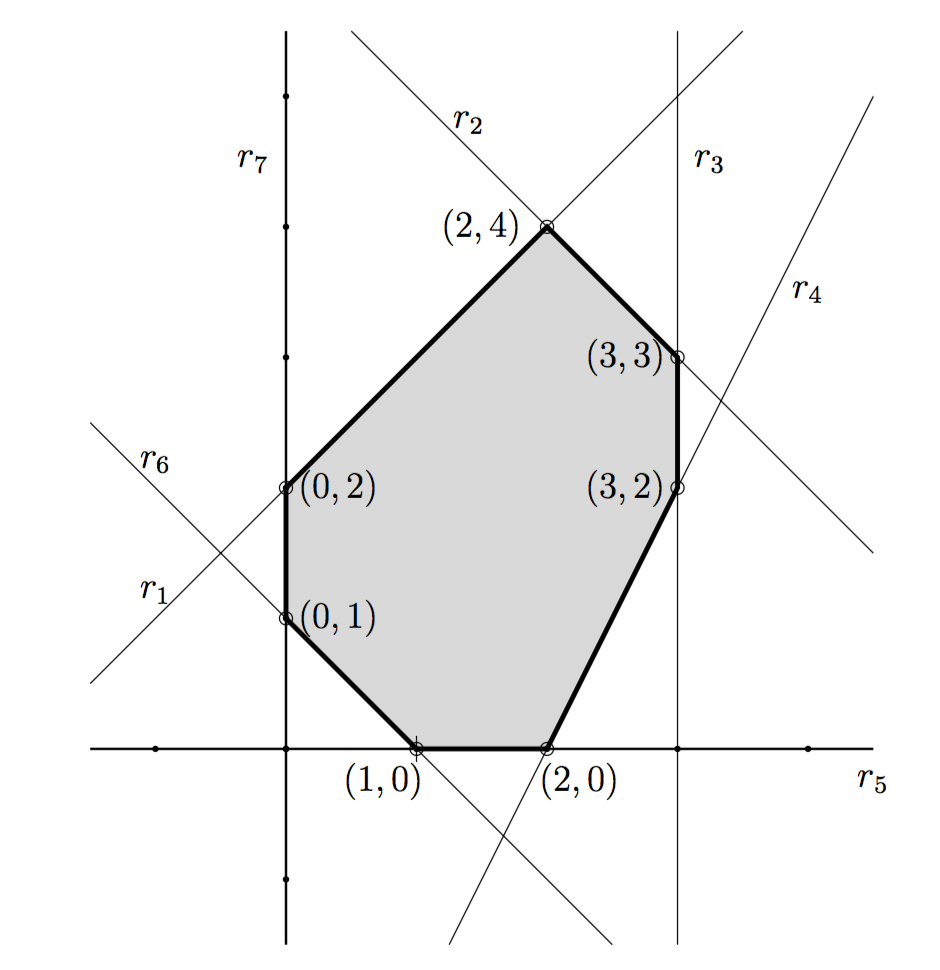
\includegraphics[height=7cm]{ex1}
\end{figure}
\end{frame}


\begin{frame}
\frametitle{Ejemplos de PL}
$R$ en este caso es un pol\'igono cerrado. Las soluciones siempre se encuentran en los extremos de la regi\'on factible, por tanto se evaluar\'a la funci\'on objetivo $Z=3x_1+x_2$ en los v\'ertices de $R$:
\[Z(0,1) = 1;\ \ \ Z(0,2) = 2;\ \ \ Z(2,4) = 10;\ \ \ Z(3,3) = 12;\]
\[Z(3,2) = 11;\ \ \ Z(2,0) = 6;\ \ \ Z(1,0) = 3.\]
Por tanto el m\'aximo se alcanza en el punto $(3,3)$ y vale $Z=12$.
\end{frame}



\begin{frame}
\frametitle{Ejemplos de PL}
\begin{block}{Ejemplo 2}
Maxim\'icese la funci\'on $Z=x_1+x_2$ bajo las restricciones:
\[\left\{\begin{array}{l}-x_1 + x_2 \leq 2 \\x_1+x_2\leq 6 \\x_1\leq 3 \\2x_1-x_2\leq 4 \\-x_2\leq 0 \\-x_1-x_2\leq -1 \\-x_1\leq 0\end{array}\right.\]
\end{block}
\end{frame}


\begin{frame}
\frametitle{Ejemplos de PL}
Obs\'ervese que el conjunto de restricciones es el mismo que el del ejemplo anterior, por tanto la regi\'on factible ser\'a la misma.
 \begin{figure}[h]
\label{fig:ejemplo 2}
\centering
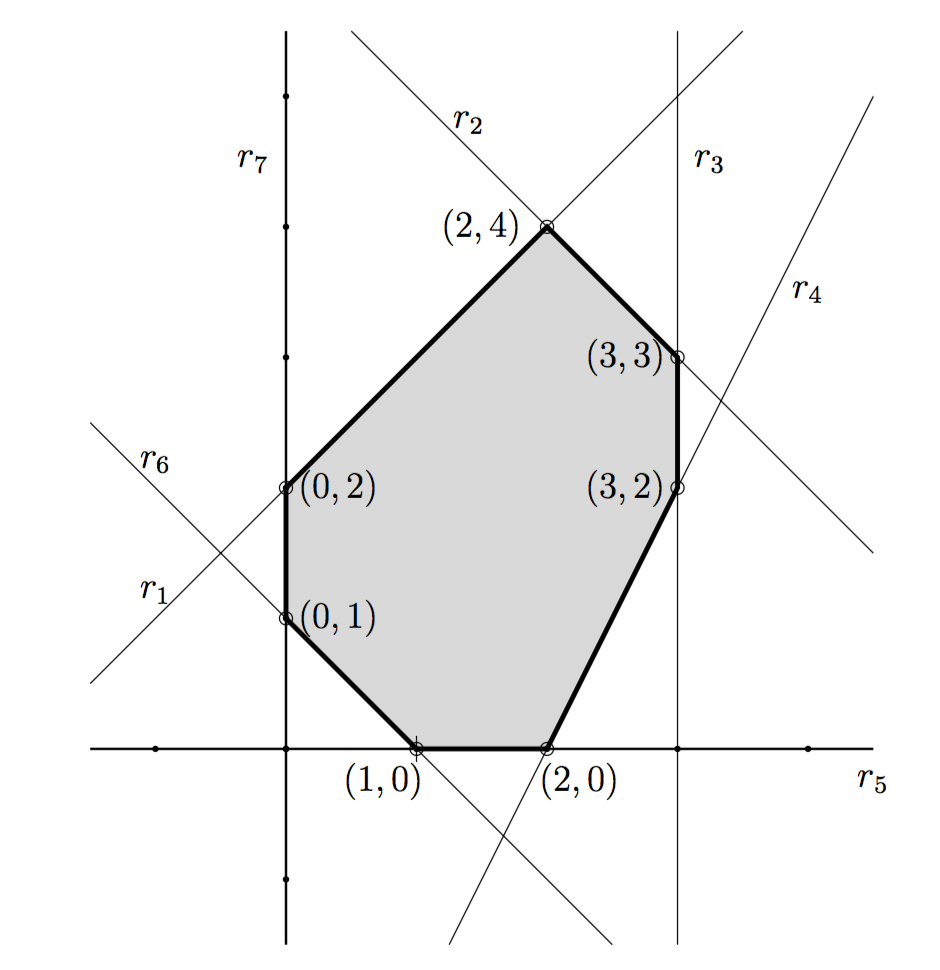
\includegraphics[height=5cm]{ex1}
\end{figure}
\end{frame}





\begin{frame}
\frametitle{Ejemplos de PL}
El m\'aximo se alcanza en los puntos $(2,4)$ y $(3,3)$, entonces todos los puntos del segmento que une estos dos puntos son m\'aximos globales.
\end{frame}

\begin{frame}
\frametitle{Ejemplos de PL}
\begin{block}{Ejemplo 3}
Maxim\'icese la funci\'on $Z=3x_1+x_2$ bajo las restricciones:
\[\left\{\begin{array}{l}-x_1 + x_2 \leq 2 \\-x_2\leq 0 \\-x_1-x_2\leq -1 \\-x_1\leq 0\end{array}\right.\]
\end{block}
\end{frame}


\begin{frame}
\frametitle{Ejemplos de PL}
En este caso se puede observar que la regi\'on factible no est\'a acotada en la direcci\'on de crecimiento de la funci\'on objetivo.
\begin{figure}[h]
\label{fig:ejemplo 3}
\centering
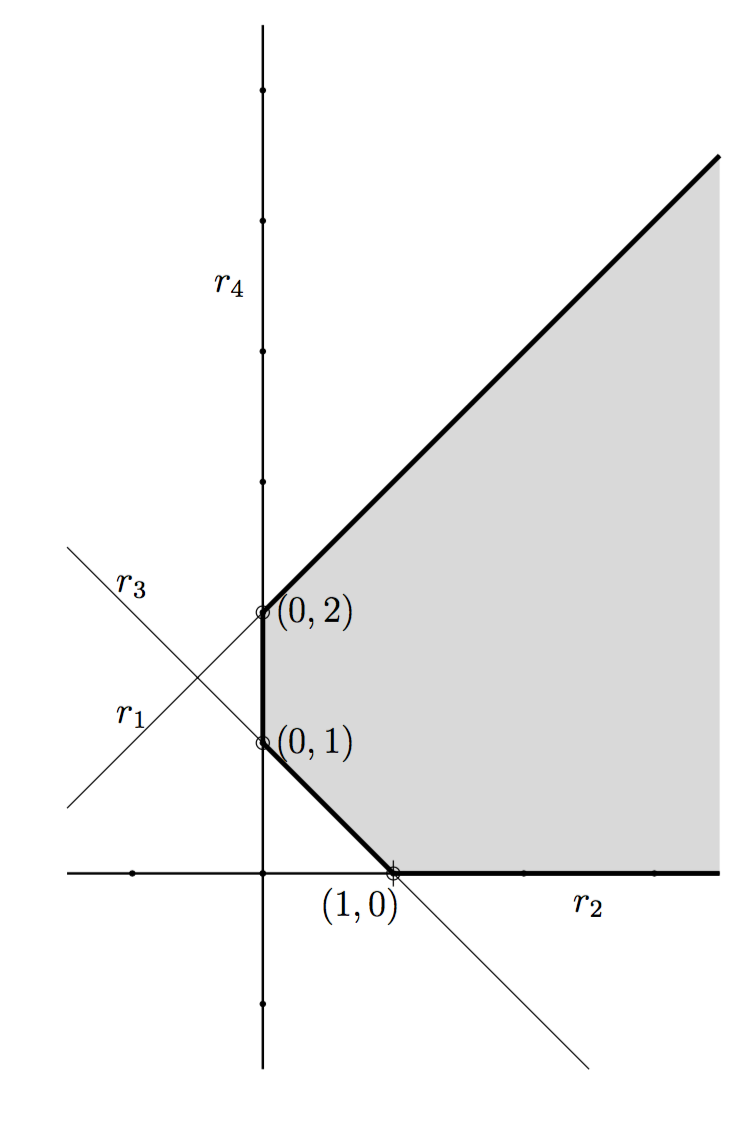
\includegraphics[height=7cm]{ex3}
\end{figure}
\end{frame}


\begin{frame}
\frametitle{Ejemplos de PL}
\begin{block}{Ejemplo 4}
Minim\'icese la funci\'on $Z=0.6x_1+x_2$ bajo las restricciones:
\[\left\{\begin{array}{l}10x_1 + 4x_2 \geq 20 \\5x_1+5x_2\geq 20 \\2x_1+6x_2\geq 12 \\x_1\geq 0\\ x_2\geq 0 \end{array}\right.\]
\end{block}
\end{frame}




\begin{frame}
\frametitle{Ejemplos de PL}
En este caso la regi\'on factible no est\'a acotada pero la funci\'on alcanza el m\'inimo en el punto $(3,1)$ y vale $Z=2.8$.
 \begin{figure}[h]
\label{fig:ejemplo 4}
\centering
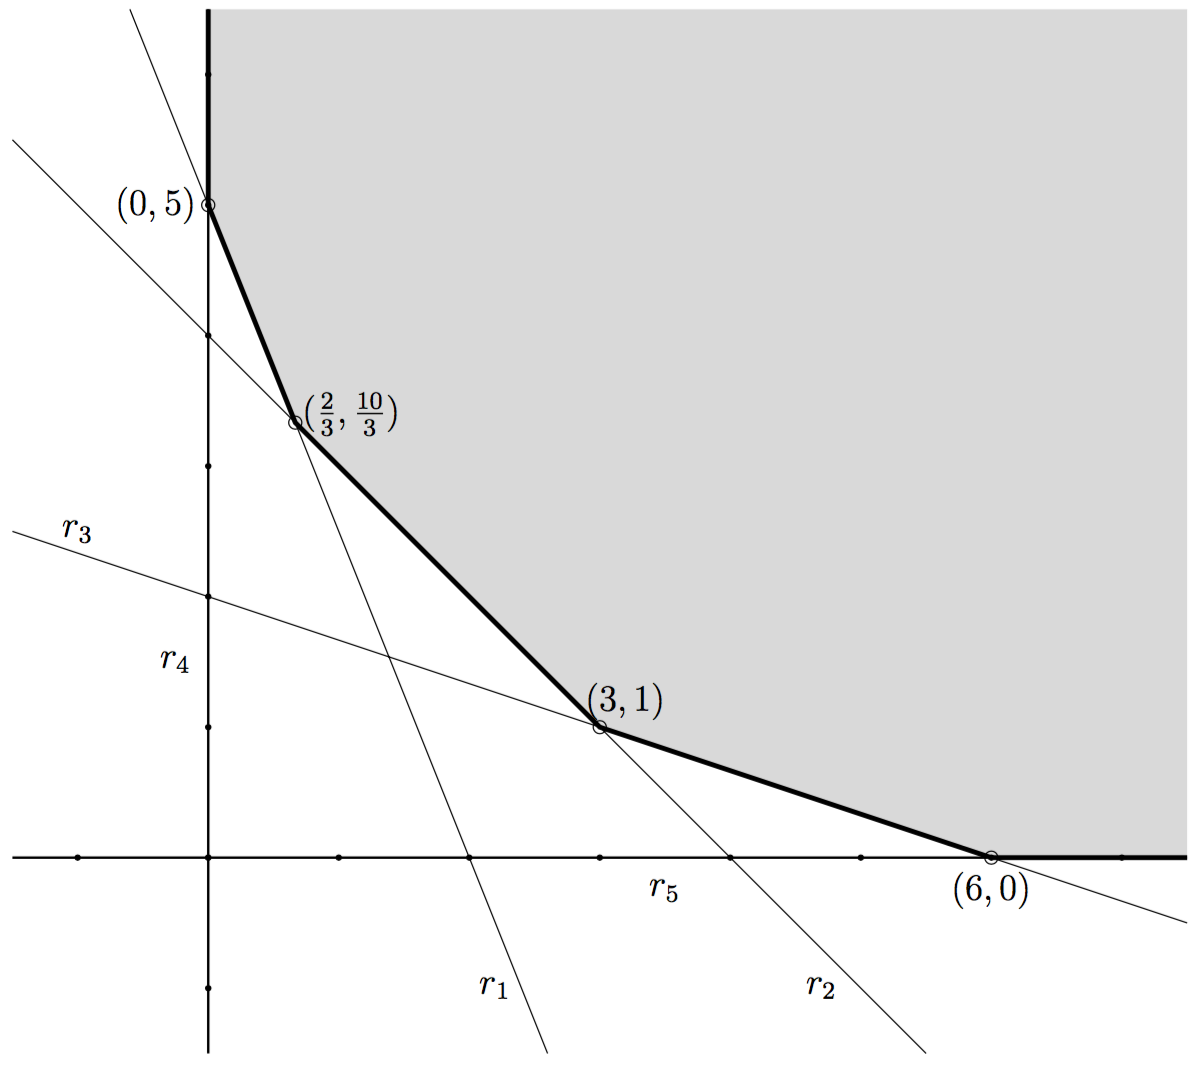
\includegraphics[height=6cm]{ex4}
\end{figure}
\end{frame}



\begin{frame}
\frametitle{Ejemplos de PL}
\begin{block}{Ejemplo 5}
Minim\'icese la funci\'on $Z=2x_1-3x_2$ bajo las restricciones:
\[\left\{\begin{array}{l}x_1-2x_2 \geq 4 \\2x_1-4x_2\leq -6 \\x_1\geq 0\\ x_2\geq 0 \end{array}\right.\]
\end{block}
En este caso, la regi\'on factible es $R=\emptyset$; es decir, el problema no tiene soluci\'on. 
\end{frame}

\subsection{Forma est\'andar de un PPL}

\begin{frame}
\frametitle{El PPL}
\begin{block}{Forma est\'andar}
Para describir un PPL, se necesita:
\begin{enumerate}
\item Un vector $c=(c_1,c_2,\cdots, c_n)\in \mathbb R^n$.
\item Un vector $b=(b_1,b_2,\cdots, b_n)\in \mathbb R^n$ con $b_i\geq 0$ para todo $i=1,\cdots, m$.
\item Una matriz $A = (a_{ij})_{m\times n}$.
\end{enumerate}
Con estos elementos, el problema lineal asociado en forma est\'andar tiene la forma siguiente:
\[Min(Max)\ Z = cX\]
Bajo las restricciones $AX=B$, donde:
\end{block}
\end{frame}



\begin{frame}
\frametitle{El PPL}
\begin{block}{Forma est\'andar}
\[X=\left(\begin{array}{l}x_1\\ x_2\\ \vdots \\ x_n \end{array}\right)\]
Con $x_j\geq 0$ para todo $j=i\cdots, n$ y:
\[B=\left(\begin{array}{l}b_1\\ b_2\\ \vdots \\ b_m \end{array}\right)\]
Con $b_i\geq 0$ para todo $i=1\cdots, m$. Normalmente $n\geq m$.
\end{block}
\end{frame}



\begin{frame}
\frametitle{El PPL}
\begin{block}{Definici\'on}
D\'icese que un PPL est\'a en forma est\'andar si:
\begin{enumerate}
\item Es de minimizaci\'on o de maximizaci\'on.
\item Solo incluye restricciones de igualdad.
\item $b_i\geq 0$ para todo $i=1,\cdots, m$.
\item $x_j\geq 0$ para todo $j=i,\cdots, n$.
\end{enumerate}
\end{block}
\end{frame}

\begin{frame}
\frametitle{Transformaci\'on de un PPL a forma est\'andar}
Cualquiera que sea el PPl se puede transformar a la forma est\'andar. V\'ease como:
\begin{block}{Paso 1: transformar las variables en no negativas}
Las variables no restringidas en signo se pueden expresar como diferencia de dos variables no negativas. Se define:
\[x_i^{+} = max\{0,x_i\}\]
\[x_i^{-} = max\{0,-x_i\}\]
Se satisface que $x_i^{+}, x_i^{-}\geq 0$ i $x_i = x_i^{+}-x_i^{-}$.
\end{block}
\end{frame}



\begin{frame}
\frametitle{Transformaci\'on de un PPL a forma est\'andar}
\begin{block}{Paso 2: transformar las restricciones de desigualdad en igualdades}
Las restricciones de desigualdad se pueden transformar en restricciones de igualdad equivalentes introduciendo nuevas variables denominadas variables compensatorias:
Si $a_{i1}x_1+a_{i2}x_2+\cdots+a_{in}x_n\leq b_i$, entonces existe una variable $x_{n+1}\geq 0$ tal que:
\[a_{i1}x_1+a_{i2}x_2+\cdots+a_{in}x_n+x_{n+1} = b_i\]
Si $a_{i1}x_1+a_{i2}x_2+\cdots+a_{in}x_n\geq b_i$, entonces existe una variable $x_{n+1}\geq 0$ tal que:
\[a_{i1}x_1+a_{i2}x_2+\cdots+a_{in}x_n-x_{n+1} = b_i\]
\end{block}
\end{frame}




\begin{frame}
\frametitle{Transformaci\'on de un PPL a forma est\'andar}
\begin{block}{Paso 3: maximizar es lo mismo que minimizar}
Un problema de maximizaci\'on $Z_{max} = cX$ es equivalente a minimizar $Z_{min} = -cX$ (y viceversa) si ambos problemas verifican el mismo conjunto de restricciones.
\end{block}
\end{frame}

\begin{frame}
\frametitle{Transformaci\'on de un PPL a forma est\'andar}
\begin{block}{Paso 4: no negatividad de los t\'erminos independientes}
Toda restricci\'on con t\'ermino independiente $b_i<0$ se puede transformar en otra con t\'ermino independiente no negativo multiplicando toda la restricci\'on por $-1$.
\end{block}
\end{frame}

\begin{frame}
\frametitle{Transformaci\'on de un PPL a forma est\'andar}
\begin{block}{Ejemplo 1}
Encu\'entrese $max\ Z = 2x_1-3x_2+5x_3$ bajo las restricciones:
\[\left\{\begin{array}{l}x_1+x_2 \leq 2 \\3x_1+x_2-x_3\geq 3 \\x_1,x_2,x_3\geq 0 \end{array}\right.\]

\end{block}
\end{frame}



\begin{frame}
\frametitle{Transformaci\'on de un PPL a forma est\'andar}
Para resolverlo se escribir\'a en forma de m\'aximo. Obs\'ervese que todas las variables son no negativas. Se tendr\'an que transformar las restricciones de desigualdad en igualdades, as\'i habr\'a que a\~nadir variables compensatorias. En forma est\'andar ser\'a:
\[max\ Z = 2x_1-3x_2+5x_3+0x_4+0x_5\]
Bajo las restricciones:

\[\left\{\begin{array}{l}x_1+x_2 +x_4  = 2 \\3x_1+x_2-x_3-x_5 = 3 \\x_1,x_2,x_3, x_4, x_5\geq 0 \end{array}\right.\]

\end{frame}



\begin{frame}
\frametitle{Transformaci\'on de un PPL a forma est\'andar}
Si se quisiese el mismo problema en forma est\'andar de m\'inimo, ser\'ia:
\[min\ Z = -2x_1+3x_2-5x_3+0x_4+0x_5\]
Bajo las restricciones:
\[\left\{\begin{array}{l}x_1+x_2 +x_4  = 2 \\3x_1+x_2-x_3-x_5 = 3 \\x_1,x_2,x_3, x_4, x_5\geq 0 \end{array}\right.\]

\end{frame}



\begin{frame}
\frametitle{Transformaci\'on de un PPL a forma est\'andar}
\begin{block}{Ejemplo 2}
Encu\'entrese $max\ Z = 2x_1-3x_2+5x_3$ bajo las restricciones:
\[\left\{\begin{array}{l}x_1+x_2 \leq 2 \\3x_1+x_2-x_3\geq 3 \\x_1,x_2\geq 0 \end{array}\right.\]

\end{block}
\end{frame}


\begin{frame}
\frametitle{Transformaci\'on de un PPL a forma est\'andar}
Obs\'ervese que esta vez la variable $x_3$ no est\'a restringida en signo. Habr\'a que escribir $x_3 = x_6-x_7$ con $x_6 = x_3^{+}\geq 0$ y $x_7 = x_3^{-}\geq 0$. As\'i el problema en forma est\'andar ser\'a:
\[max\ Z = 2x_1-3x_2+5(x_6-x_7)+0x_4+0x_5\]
Bajo las restricciones:
\[\left\{\begin{array}{l}x_1+x_2 +x_4  = 2 \\3x_1+x_2-(x_6-x_7)-x_5 = 3 \\x_1,x_2, x_4, x_5, x_6, x_7\geq 0 \end{array}\right.\]

\end{frame}




\begin{frame}
\frametitle{Transformaci\'on de un PPL a forma est\'andar}
\begin{block}{Ejemplo 3}
Encu\'entrese $max\ Z = 3x_1-x_3$ bajo las restricciones:
\[\left\{\begin{array}{l}x_1+x_2+x_3 = 1 \\x_1-x_2-x_3\leq 1\\ x_1+x_3\geq -1 \\x_1\geq 0 \end{array}\right.\]

\end{block}
\end{frame}



\begin{frame}
\frametitle{Transformaci\'on de un PPL a forma est\'andar}
Como todas las variables han de ser no negativas habr\'a que pasar a:
\[x_2 = y_2-z_2; \ \ y_2 = x_2^{+},z_2 = x_2^{-}\]
\[x_3 = y_3-z_3; \ \ y_3 = x_3^{+},z_3 = x_3^{-}\]
Con $y_2,z_2,y_3,z_3\geq 0$. N\'otese que el t\'ermino independiente de la tercera restricci\'on es negativo, entonces se multiplica por $-1$. El problema inicial ser\'a:
\[max\ Z = max\ Z = 3x_1-y_3+z_3\]
Bajo las restricciones:

\[\left\{\begin{array}{l}x_1+y_2-z_2+y_3-z_3  = 1 \\x_1-y_2+z_2-y_3+z_3\leq 1 \\ -x_1-y_3+z_3\leq 1\\x_1,y_2,z_2, y_3, z_3\geq 0 \end{array}\right.\]

\end{frame}




\begin{frame}
\frametitle{Transformaci\'on de un PPL a forma est\'andar}
Ahora solo falta transformar las restricciones de desigualdad en restricciones de igualdad:
\[\left\{\begin{array}{l}x_1+y_2-z_2+y_3-z_3  = 1 \\x_1-y_2+z_2-y_3+z_3 +u_1=  1 \\ -x_1-y_3+z_3 + u_2 = 1\\x_1,y_2,z_2, y_3, z_3, u_1, u_2\geq 0 \end{array}\right.\]
\end{frame}


\subsection{Soluciones b\'asicas de un PPL}
\begin{frame}
\frametitle{Soluciones b\'asicas de un PPL}
Sup\'ongase que un PPL viene dado en forma est\'andar $min(max)\ Z = cX$ bajo las restricciones $AX=B$ donde:
\[X=(x_1,x_2,\cdots, x_n)^t, \ \ x_j\geq 0 \ \forall i = i,\cdots, n\]
\[B=(b_1,b_2,\cdots, b_m)^t, \ \ b_i\geq 0 \ \forall i =1,\cdots, m\]
\[A=(a_{ij})_{m\times n}\]
Se puede suponer sin p\'erdida de generalidad que $rang(A) = m$, ya que $m\leq n$ y que el sistema $AX=B$ tiene soluci\'on. En cualquier otro caso, o bien el sistema es equivalente a otro sistema compatible con menos ecuaciones o bien el sistema es incompatible.
\end{frame}



\begin{frame}
\frametitle{Soluciones b\'asicas de un PPL}
Sea $A$ la matriz anterior, entonces:
\begin{block}{Definici\'on}
\begin{itemize}
\item Se denomina b\'asica de $A$ a toda matriz de orden $m$, $M_b$ de rango $m$ extra\'ida de $A$.
\item $M_b$ es b\'asica factible si es b\'asica y satisface $M_b^{-1}B\geq 0$.

\end{itemize}
\end{block}
\end{frame}




\begin{frame}
\frametitle{Soluciones b\'asicas de un PPL}
\begin{block}{Definici\'on}
Sea $X_b$ el vector de las variables asociadas a las columnas de $M_b$, estas variables se denominan b\'asicas y las dem\'as variables no b\'asicas. Si se asigna el valor cero a las variables no b\'asicas $X_N$, el sistema $AX=B$ se puede escribir como:
\[(M_b\ \ |\ \ X_N) \left(\begin{array}{c}X_b \\0\end{array}\right) = B\]
Donde $M_bX_b = B$ y, como $M_b$ es invertible, $X_b = M_b^{-1}B$ es la soluci\'on b\'asica asociada a $M_b$. Si adem\'as $M_b$ es una matriz b\'asica factible, su soluci\'on b\'asica es factible.
\end{block}
\end{frame}




\begin{frame}
\frametitle{Soluciones b\'asicas de un PPL}
\begin{block}{Ejemplo 1}
Encu\'entrense las soluciones b\'asicas del sistema.
\[\left\{\begin{array}{ccc}x_1+2x_2+x_3 & = & 8 \\x_1+3x_2-x_3 & = & 12\end{array}\right.\]
\end{block}
\end{frame}




\begin{frame}
\frametitle{Ejemplo 1}
Las matrices $A$ y $B$ son:
\[A=\left(\begin{array}{ccc}1&2&1 \\1&3&-1\end{array}\right)\]
\[B=\left(\begin{array}{c}8 \\12\end{array}\right)\]
\end{frame}




\begin{frame}
\frametitle{Ejemplo 1.1}
Si se considera:
\[M_b=\left(\begin{array}{cc}1&2 \\1&3\end{array}\right)\]
Las variables son $x_1,x_2$ y la variable no b\'asica $x_3=0$, entonces:
\[X_b = M_b^{-1} B= \left(\begin{array}{cc}3&-2 \\-1&1\end{array}\right) \left(\begin{array}{c}8 \\12\end{array}\right) = \left(\begin{array}{c}0 \\4\end{array}\right)\]
As\'i $(x_1,x_2) = (0,4)$ es una soluci\'on b\'asica factible.
\end{frame}

\begin{frame}
\frametitle{Ejemplo 1.2}
Si tomamos como matriz b\'asica:
\[M_b=\left(\begin{array}{cc}1&1 \\1&-1\end{array}\right)\]
Las variables son $x_1,x_3$ y la variable no b\'asica $x_2=0$, entonces:
\[X_b = M_b^{-1} B= \left(\begin{array}{cc}1/2&1/2 \\1/2&-1/2\end{array}\right) \left(\begin{array}{c}8 \\12\end{array}\right) = \left(\begin{array}{c}10 \\-2\end{array}\right)\]
En este caso se obtiene una soluci\'on b\'asica no factible ($x_3<0$)
\end{frame}

\begin{frame}
\frametitle{Ejemplo 1.3}
Si se toma como matriz b\'asica:
\[M_b=\left(\begin{array}{cc}2&1 \\3&-1\end{array}\right)\]
Las variables son $x_2,x_3$ y la variable no b\'asica $x_1=0$, entonces:
\[X_b = M_b^{-1} B= \left(\begin{array}{cc}1/5&1/5 \\3/5&-2/5\end{array}\right) \left(\begin{array}{c}8 \\12\end{array}\right) = \left(\begin{array}{c}4 \\0\end{array}\right)\]
As\'i $(x_2,x_3) = (4,0)$ es una soluci\'on b\'asica factible.
\end{frame}


\begin{frame}
\frametitle{Ejemplo 1}
El n\'umero de soluciones b\'asicas factibles de un PPL acotado con un n\'umero finito de restricciones es siempre finito y a cada una le corresponde un punto extremo de la regi\'on factible.
\end{frame}




\begin{frame}
\frametitle{Soluciones b\'asicas de un PPL}
\begin{block}{Teorema}
Sea:
\[R=\{x=(x_1,x_2,\cdots, x_n) : AX=B, x_j\geq 0\ j=1\cdots, n\}\]
Con $A=(a_{ij})_{m\times n}$ y $rang(A) = m$, entonces $x\in \mathbb R^n$ es un punto extremo de $R$ si y solo si $A$ se puede descomponer como $A=(M_b \ | \ X_N)$ tal que:
 \[X = \left(\begin{array}{c}X_b \\X_N\end{array}\right) \left(\begin{array}{c}M_b^{-1} B \\0\end{array}\right) \]
Donde $M_b$ es una matriz de orden $m$ invertible, extra\'ida de $A$ que satisface $M^{-1}B\geq 0$

\end{block}
\end{frame}





\begin{frame}
\frametitle{Soluciones b\'asicas de un PPL}
\begin{block}{Observaci\'on}
Recu\'erdese que si $M_b$ es una matriz de orden $m$ invertible, es equivalente por filas a la matriz identidad $I_m$ o a cualquier otra matriz de orden $m$, las columnas de la cual son los vectores unitarios: $e_1=(1,0,\cdots,0),e_2=(0,1,\cdots,0),\cdots,e_m=(0,0,\cdots,1)$ no necesariamente en este orden:
 \[I_m \sim \left(\begin{array}{ccc}1&0&0 \\0&1&0\\ 0&0&1\end{array}\right)  
 \sim \left(\begin{array}{ccc}0&1&0 \\1&0&0\\ 0&0&1\end{array}\right) 
 \sim \left(\begin{array}{ccc}0&1&0 \\0&0&1\\ 1&0&0\end{array}\right) \sim \cdots\]
\end{block}
\end{frame}



\begin{frame}
\frametitle{Soluciones b\'asicas de un PPL}
\begin{block}{Teorema. Propiedad fundamental de la programaci\'on lineal}
Si un PPL tiene una soluci\'on \'optima, esta es una soluci\'on b\'asica factible. 
\end{block}
Por tanto, para hallar el \'optimo de un PPL se encontrar\'a en el conjunto de soluciones factibles.
\end{frame}


\section{El m\'etodo del s\'implex}

\begin{frame}
\frametitle{El m\'etodo del s\'implex}

Es un procedimiento algebraico (no geom\'etrico) mediante el cual se pasa de una soluci\'on b\'asica factible inicial (o cualquier otra) a una soluci\'on b\'asica factible adyacente, mejorando, o al menos, no empeorando el valor de la funci\'on objetivo.

Existen muchas versiones del m\'etodo s\'implex y todas pretenden lo mismo: encontrar la soluci\'on \'optima de un PPL.

Para encontrar este \'optimo se emplean unas tablas. Se parte de una tabla inicial y se van transformando los valores de la tabla hasta llegar a la soluci\'on \'optima.

En este curso se aplicar\'a el m\'etodo revisado del s\'implex que incluye la funci\'on objetivo en las tablas. En el m\'etodo del s\'implex se toma como matriz b\'asica factible inicial la matriz identidad y cualquier otra matriz b\'asica factible obtenida a partir de la matriz identidad haciendo intercambios de filas.
\end{frame}

\subsection{Un ejemplo para comenzar}
\begin{frame}
\frametitle{El m\'etodo del s\'implex}
\begin{block}{Ejemplo del s\'implex}
Encu\'entrese $max\ Z = 40x_1+30x_2$ bajo las restricciones:
\[\left\{\begin{array}{ccc}x_1 & \leq & 16 \\x_2 & \leq & 8 \\x_1+2x_2 & \leq & 24 \\x_1,x_2 & \geq & 0\end{array}\right.\]
\end{block}
\end{frame}


\begin{frame}
\frametitle{El m\'etodo del s\'implex}
Si se resuleve gr\'aficamente obteniendo la regi\'on factible con v\'ertices $(0, 0), (16, 0), (16, 4), (8, 8), (0, 8)$ y se eval\'ua $Z$ en estos v\'ertices se obtiene que el m\'aximo se alcanza en el punto $(16, 4)$ y vale $760$.
\end{frame}


\begin{frame}
\frametitle{El m\'etodo del s\'implex}
Para aplicar el m\'etodo del s\'implex se han de hacer una serie de pasos:
\end{frame}



\begin{frame}
\frametitle{El m\'etodo del s\'implex - Paso 1}
Se ha de escribir el problema de forma est\'andar de m\'aximo, que ser\'a el mismo que denota el sistema:
\[\left.\begin{array}{rrrrrrrr}
Z & -40x_1 & -30x_2 & +0s_1 & +0s_2& +0s_3 & = & 0 \\
 &  x_1 &  & +s_1 & &  & = & 16 \\
 &  & x_2 &  & +s_2&  & = & 8 \\
  & x_1 & +2x_2 &  & & +s_3 & = & 24 \end{array}\right.\]
Con $x_1,x_2,s_1,s_2,s_3\geq 0$.
\end{frame}

\begin{frame}
\frametitle{El m\'etodo del s\'implex - Paso 1}
Se puede construir la tabla:
\begin{tabular}{ |p{1cm}||p{0.8cm}|p{0.8cm}|p{0.8cm}|p{0.8cm}|p{0.8cm}|p{0.8cm}|p{1.6cm}|  }
 \hline
 & Z & $x_1$ & $x_2$ & $s_1$& $s_2$ & $s_3$ & Constantes \\
 \hline
fila 1 &1 & -40 & -30 & 0& 0& 0 & 0 \\
fila 2 & 0 &  1 & 0 & 1 & 0 & 0 & 16 \\
fila 3 & 0 & 0 & 1 & 0 & 1 & 0  & 8 \\
fila 4 &  0 & 1 & 2 & 0 &0 & 1  & 24\\
      \hline
\end{tabular}

La matriz b\'asica factible inicial (matriz identidad) corresponde a las variables b\'asicas, en este caso a las variables compensatorias $s_1,s_2,s_3$ y las variables no b\'asicas son $x_1=x_2=0$.

\end{frame}





\begin{frame}
\frametitle{El m\'etodo del s\'implex - Paso 1}
Teniendo en cuenta tambi\'en la fila 1 de la tabla, se puede expresar el sistema:
\[\left(\begin{array}{cccc}
1&0&0&0 \\
0&1&0&0 \\
0&0&1&0 \\
0&0&0&1 \\
 \end{array}\right)
 \left(\begin{array}{c}
Z\\s_1\\s_2\\s_3
 \end{array}\right) = 
  \left(\begin{array}{c}
0\\16\\8\\24
 \end{array}\right) 
 \]

Que corresponde a $s_1=16, s_2 = 8, s_3 = 24$ y $Z=0$ (con $(x_1,x_2) = (0,0)$. N\'otese que el punto $(0,0)$ es un v\'ertice de la regi\'on factible.
\end{frame}



\begin{frame}
\frametitle{El m\'etodo del s\'implex - Paso 2}
\begin{itemize}
\item Se busca la columna que en la fila 1 tiene la entrada negativa con mayor valor absoluto (columna pivote).
\item Se dividen las constantes por los valores positivos de la columna pivote y se elige el m\'inimo, la fila correspondiente a este m\'inimo ser\'a la fila pivote.
\item El elemento que est\'e en la instersecci\'on de la fila y la columna pivotes debe corresponderse con la nueva variable b\'asica. N\'otese que en nuestro caso la columna pivote es la segunda fila y la fila pivote es la que correspondr\'a a la nueva al m\'inimo entre $16/1$ y $24/1$, es decir, la fila 2. Por lo tanto el pivote es 1 y le corresponde la variable $x_1$.
\item Se transforma la tabla inicial de manera que la columna pivote sea un vector unitario (todos los elementos de la columna han de ser nulos salvo el pivote que debe ser $1$). 
\end{itemize}
\end{frame}


\begin{frame}
\frametitle{El m\'etodo del s\'implex - Paso 2}
Por tanto, si se hace $f_1+40f_2, f_4-f_2$ se obtiene la nueva tabla:
\begin{tabular}{ |p{1cm}||p{0.8cm}|p{0.8cm}|p{0.8cm}|p{0.8cm}|p{0.8cm}|p{0.8cm}|p{1.6cm}|  }
 \hline
 & Z & $x_1$ & $x_2$ & $s_1$& $s_2$ & $s_3$ & Constantes \\
 \hline
fila 1 &1 & 0 & -30 & 40& 0& 0 & 640 \\
fila 2 & 0 &  1 & 0 & 1 & 0 & 0 & 16 \\
fila 3 & 0 & 0 & 1 & 0 & 1 & 0  & 8 \\
fila 4 &  0 & 0 & 2 &-1 &0 & 1  & 8\\
      \hline
\end{tabular}
\end{frame}






\begin{frame}
\frametitle{El m\'etodo del s\'implex - Paso 2}
De la tabla se puede extraer el sistema b\'asico:
\[\left(\begin{array}{cccc}
1&0&0&0 \\
0&1&0&0 \\
0&0&1&0 \\
0&0&0&1 \\
 \end{array}\right)
 \left(\begin{array}{c}
Z\\x_1\\s_2\\s_3
 \end{array}\right) = 
  \left(\begin{array}{c}
640\\16\\8\\8
 \end{array}\right) 
 \]

Que corresponde a $x_1=16, s_2 = 8, s_3 = 8$ y $Z=640$ (con $x_2=0, s_2 = 0$). N\'otese que el punto $(16,0)$ es otro v\'ertice de la regi\'on factible.
\end{frame}


\begin{frame}
\frametitle{El m\'etodo del s\'implex - Paso 3}
Como en la fila 1  todav\'ia hay un n\'umero negativo, la soluci\'on se puede mejorar. Iterando el paso 2 anterior:
\begin{itemize}
\item La nueva variable b\'asica es $x_2$. 
\item Si se hace el m\'inimo entre $8/1$ y $8/2$, se obtiene que el pivote est\'a en la fila $4$.
\item El pivote es $2$ y por tanto se dividir\'a la fila pivote por $2$ para obtener el pivote 1.
\item Finalmente, se hacen ceros mediante la resta de elementos de la columna pivote.
\end{itemize}
\end{frame}



\begin{frame}
\frametitle{El m\'etodo del s\'implex - Paso 3}
Por tanto, si se hace $f_1+30f_4, f_3-f_4$ se obtiene la nueva tabla:
\begin{tabular}{ |p{1cm}||p{0.8cm}|p{0.8cm}|p{0.8cm}|p{0.8cm}|p{0.8cm}|p{0.8cm}|p{1.6cm}|  }
 \hline
 & Z & $x_1$ & $x_2$ & $s_1$& $s_2$ & $s_3$ & Constantes \\
 \hline
fila 1 &1 & 0 & 0 & 25& 0& 15 & 760 \\
fila 2 & 0 &  1 & 0 & 1 & 0 & 0 & 16 \\
fila 3 & 0 & 0 & 0 & 1/2 & 1 & -1/2  & 4 \\
fila 4 &  0 & 0 & 1 &-1/2 &0 & 1/2  & 4\\
      \hline
\end{tabular}
\end{frame}




\begin{frame}
\frametitle{El m\'etodo del s\'implex - Paso 3}
De la tabla se puede extraer el sistema b\'asico:
\[\left(\begin{array}{cccc}
1&0&0&0 \\
0&1&0&0 \\
0&0&1&0 \\
0&0&0&1 \\
 \end{array}\right)
 \left(\begin{array}{c}
Z\\x_1\\ s_2\\x_2
 \end{array}\right) = 
  \left(\begin{array}{c}
760\\16\\4\\4
 \end{array}\right) 
 \]

Que se corresponde con $x_1=16, x_2 = 4, s_2 = 4$ y $Z=760$ (donde $s_1=0, s_3 = 0$). N\'otese que el punto $(16,4)$ es otro v\'ertice de la regi\'on factible. 

En la fila 1 ya no quedan n\'umeros negativos, por tanto la soluci\'on no se puede mejorar.
\end{frame}

\subsection{El m\'etodo del s\'implex en problemas de minimizaci\'on}

\begin{frame}
\frametitle{El m\'etodo del s\'implex en problemas de minimizaci\'on}
En problemas de minimizaci\'on no se puede aplicar directamente el m\'etodo que se ha descrito en el apartado anterior. V\'ease c\'omo proceder en este caso con el siguiente ejemplo:
\end{frame}


\begin{frame}
\frametitle{El m\'etodo del s\'implex en problemas de minimizaci\'on}
\begin{block}{Ejemplo 2 del s\'implex}
Encu\'entrese $min\ Z =x_1+4x_2$ bajo las restricciones:
\[\left\{\begin{array}{ccc}x_1+2x_2 & \geq & 8 \\3x_1+2x_2 & \geq & 12 \\x_1,x_2 & \geq & 0\end{array}\right.\]
\end{block}
\end{frame}


\begin{frame}
\frametitle{El m\'etodo del s\'implex en problemas de minimizaci\'on}
Si se escribe en forma est\'andar de m\'inimo, queda:
\[min\ Z = x_1+4x_2+0s_1+0s_2\]
Bajo las restricciones:
\[\left(\begin{array}{rrrr}1&2&-1&0 \\3&2&0&-1\end{array}\right)
\left(\begin{array}{c}x_1\\ x_2\\ s_1\\ s_2\end{array}\right) = 
\left(\begin{array}{c}8\\ 12 \\ \end{array}\right)\]
Con $x_1,x_2,s_1,s_2\geq 0$
\end{frame}

\begin{frame}
\frametitle{El m\'etodo del s\'implex en problemas de minimizaci\'on}
Se puede observar que de la matriz de coeficientes no se puede extraer la matiz identidad como matriz b\'asica factible inicial. Se podr\'ia extraer la matriz:
\[\left(\begin{array}{cc}-1&0 \\0&-1\end{array}\right)\]
Que corresponden a las variables b\'asicas $s_1,s_2$. La soluci\'on $s_1 = -8, s_2 = -12$, que resulta una soluci\'on b\'asica no factible. Consecuentemente se ha de buscar una manera de obtener una soluci\'on b\'asica factible inicial. Esta se obtiene a\~nadiendo una variable artificial no negativa a cada una de las restricciones. Estas variables artificiales aparecer\'an en la funci\'on objetivo con coeficientes \textbf{grandes} respecto a los coeficientes de las variables del problema dado. 
\end{frame}

\begin{frame}
\frametitle{El m\'etodo del s\'implex en problemas de minimizaci\'on}
Una vez se a\~naden las variables compensatorias y artificiales al problema de minimizaci\'on se aplicar\'a el m\'etodo del s\'implex aplicando los paso siguientes:
\begin{enumerate}
\item Se escribe la tabla inicial del s\'implex.
\item Se transforman las columnas de las variables artificiales en vectores unitarios.
\item Se busca el pivote: de entre todas las columnas de las variables se elige la columna con la entrada positiva mayor. Para determinar la fila pivote se hace lo mismo que en el caso de la maximizaci\'on.
\end{enumerate}
\end{frame}


\begin{frame}
\frametitle{El m\'etodo del s\'implex en problemas de minimizaci\'on}
Si se considera el problema de minimizaci\'on del ejemplo anterior, una vez a\~nadidas las variables artificiales se tiene:
\[\left.\begin{array}{rrrrrrrrr}
Z & -x_1 & -4x_2 & +0s_1 & +0s_2& -100v_1 & -100 v_2 & = & 0 \\
 &  x_1 & +2x_2 & -s_1 & &  +v_1&& = & 8 \\
 & 3x_1 & +2x_2 &  & -s_2&  & +v_2 & = & 12 \\
  \end{array}\right.\]
Con $x_1,x_2,s_1,s_2,v_1,v_2\geq 0$.
\end{frame}

\begin{frame}
\frametitle{El m\'etodo del s\'implex en problemas de minimizaci\'on}
Se escribe la tabla inicial del problema:
\begin{tabular}{ |p{1cm}||p{0.8cm}|p{0.8cm}|p{0.8cm}|p{0.8cm}|p{0.8cm}|p{0.8cm}|p{1.6cm}|  }
 \hline
 Z & $x_1$ & $x_2$ & $s_1$& $s_2$ & $v_1$  & $v_2$& Constantes \\
 \hline
1 &-1 & -4 & 0 & 0& -100& -100 & 0 \\
0 & 1 &  2 & -1 & 0 & 1 & 0 & 8 \\
0 & 3 & 2 & 0 & -1 & 0 & 1  & 12 \\
 \hline
\end{tabular}
\end{frame}


\begin{frame}
\frametitle{El m\'etodo del s\'implex en problemas de minimizaci\'on}
Si se hace $f_1+100f_2+100f_3$, los vectores columna de las variables artificiales se transforma en unitarios y se obtiene la tabla:
\begin{tabular}{ |p{1cm}||p{0.8cm}|p{0.8cm}|p{0.8cm}|p{0.8cm}|p{0.8cm}|p{0.8cm}|p{1.6cm}|  }
 \hline
 Z & $x_1$ & $x_2$ & $s_1$& $s_2$ & $v_1$  & $v_2$& Constantes \\
 \hline
1 &399 & 396 & -100 & -100& 0& 0 & 2000 \\
0 & 1 &  2 & -1 & 0 & 1 & 0 & 8 \\
0 & 3 & 2 & 0 & -1 & 0 & 1  & 12 \\
 \hline
\end{tabular}
\end{frame}


\begin{frame}
\frametitle{El m\'etodo del s\'implex en problemas de minimizaci\'on}
La columna pivote corresponde a la columna de la variable $x_1$ y la fila pivote es la tercera. Se dividir\'a la fila pivote por $3$ para tener el pivote igual    a $1$ y se obtiene
\begin{tabular}{ |p{1cm}||p{0.8cm}|p{0.8cm}|p{0.8cm}|p{0.8cm}|p{0.8cm}|p{0.8cm}|p{1.6cm}|  }
 \hline
 Z & $x_1$ & $x_2$ & $s_1$& $s_2$ & $v_1$  & $v_2$& Constantes \\
 \hline
1 &399 & 396 & -100 & -100& 0& 0 & 2000 \\
0 & 1 &  2 & -1 & 0 & 1 & 0 & 8 \\
0 & 1 & 2/3 & 0 & -1/3 & 0 & 1/3  & 4 \\
 \hline
\end{tabular}
\end{frame}


\begin{frame}
\frametitle{El m\'etodo del s\'implex en problemas de minimizaci\'on}
Si ahora se hace $f_1-399f_3$ y $f_2-f_3$ se transforma la columna pivote en un vector unitario y se obtiene una nueva tabla:
\begin{tabular}{ |p{1cm}||p{0.8cm}|p{0.8cm}|p{0.8cm}|p{0.8cm}|p{0.8cm}|p{0.8cm}|p{1.6cm}|  }
 \hline
 Z & $x_1$ & $x_2$ & $s_1$& $s_2$ & $v_1$  & $v_2$& Constantes \\
 \hline
1 &0 & 130 & -100 & 33& 0& -133 & 404 \\
0 & 0 &  4/3 & -1 & 1/3 & 1 & -1/3 & 4 \\
0 & 1 & 2/3 & 0 & -1/3 & 0 & 1/3  & 4 \\
 \hline
\end{tabular}
\end{frame}



\begin{frame}
\frametitle{El m\'etodo del s\'implex en problemas de minimizaci\'on}
As\'i se puede extraer el sistema: 
\[\left(
\begin{array}{ccc}
1&0&0 \\ 0&1&0\\ 0&0&1
\end{array}
\right)
\left(
\begin{array}{c}
Z\\v_1\\x_1
\end{array}
\right) = \left(
\begin{array}{c}
404\\ 4\\ 4\end{array}
\right)
\]
Que corresponde a la soluci\'on $x_1 = 4, v_1 = 4, s_1=s_2=x_2=v_2=0$ y $Z=404$. N\'otese que en la soluci\'on aparece la variable artificial $v_1=4$, lo cual no interesa. La soluci\'on no es \'optima, todav\'ia queda en la fila 1 entradas positivas. La entrada positiva m\'as grande corresponde a la variable $x_2$, por tanto la columna correspondente a $x_2$ es la columna pivote y la fila pivote es la $2$, con pivote $4/3$.
\end{frame}





\begin{frame}
\frametitle{El m\'etodo del s\'implex en problemas de minimizaci\'on}
Si se divide la fila pivote por $4/3$ se tiene que:
\begin{tabular}{ |p{0.6cm}||p{0.8cm}|p{0.8cm}|p{0.8cm}|p{0.8cm}|p{0.8cm}|p{0.8cm}|p{1.6cm}|  }
 \hline
 Z & $x_1$ & $x_2$ & $s_1$& $s_2$ & $v_1$  & $v_2$& Constantes \\
 \hline
1 &0 & 130 & -100 & 33& 0& -133 & 404 \\
0 & 0 &  1 & -3/4 & 1/4 & 3/4 & -1/4 & 3 \\
0 & 1 & 2/3 & 0 & -1/3 & 0 & 1/3  & 4 \\
 \hline
\end{tabular}
\end{frame}


\begin{frame}
\frametitle{El m\'etodo del s\'implex en problemas de minimizaci\'on}
Se har\'a $f_1-130f_2$ y $f_3-2/3f_2$, transformando la columna pivote en un vector unitario quedar\'ia esta nueva tabla:

\begin{tabular}{ |p{0.6cm}||p{0.8cm}|p{0.8cm}|p{0.8cm}|p{0.8cm}|p{1.2cm}|p{1.2cm}|p{1.6cm}|  }
 \hline
 Z & $x_1$ & $x_2$ & $s_1$& $s_2$ & $v_1$  & $v_2$& Constantes \\
 \hline
1 &0 & 0 & -5/2 & 1/2& -195/2& -201/2 & 14 \\
0 & 0 &  1 & -3/4 & 1/4 & 3/4 & -1/4 & 3 \\
0 & 1 & 0 & 1/2 & -1/2 & -1/2 & 1/2  & 2 \\
 \hline
\end{tabular}
La soluci\'on todav\'ia no es \'optima. Si se itera el proceso se obtiene que la columna pivote corresponde a la columna de la variable $s_2$ y la fila 2 es la fila pivote, con pivote $1/4$. 

Nota: la fila 3 no puede ser pivote, ya que es un nombre negativo, y si dividi\'esemos por $-1/2$, el valor de $b_3$ se covertir\'ia en negativo tambi\'en...
\end{frame}


\begin{frame}
\frametitle{El m\'etodo del s\'implex en problemas de minimizaci\'on}
Si se divide la fila pivote por $1/4$, queda:
\begin{tabular}{ |p{0.6cm}||p{0.8cm}|p{0.8cm}|p{0.8cm}|p{0.8cm}|p{1.2cm}|p{1.2cm}|p{1.6cm}|  }
 \hline
 Z & $x_1$ & $x_2$ & $s_1$& $s_2$ & $v_1$  & $v_2$& Constantes \\
 \hline
1 &0 & 0 & -5/2 & 1/2& -195/2& -201/2 & 14 \\
0 & 0 &  4 & -3 & 1 & 3 & -1 & 12 \\
0 & 1 & 0 & 1/2 & -1/2 & -1/2 & 1/2  & 2 \\
 \hline
\end{tabular}
\end{frame}


\begin{frame}
\frametitle{El m\'etodo del s\'implex en problemas de minimizaci\'on}
Si ahora se hace $f_1-1/2f_2$ y $f_3+1/2f_2$ se transforma la columna pivote en un vector unitario y se obtiene una nueva tabla:
\begin{tabular}{ |p{0.6cm}||p{0.8cm}|p{0.8cm}|p{0.8cm}|p{0.8cm}|p{1.2cm}|p{1.2cm}|p{1.6cm}|  }
 \hline
 Z & $x_1$ & $x_2$ & $s_1$& $s_2$ & $v_1$  & $v_2$& Constantes \\
 \hline
1 &0 & -2 & -1 & 0& -99& -100 & 8 \\
0 & 0 &  4 & -3 & 1 & 3 & -1 & 12 \\
0 & 1 & 2 & -1 & 0 & 1 & 0  & 8 \\
 \hline
\end{tabular}
\end{frame}




\begin{frame}
\frametitle{El m\'etodo del s\'implex en problemas de minimizaci\'on}
As\'i es posible extraer el sistema:
\[\left(
\begin{array}{ccc}
1&0&0 \\ 0&1&0\\ 0&0&1
\end{array}
\right)
\left(
\begin{array}{c}
Z\\s_2\\x_1
\end{array}
\right) = \left(
\begin{array}{c}
8\\ 12\\ 8\end{array}
\right)
\]
Que corresponde a la soluci\'on $x_1 = 8, s_2=12, x_2=s_1= v_1 =v_2=0$ i  $Z=8$. Por tanto, la soluci\'on \'optima es $(x_1,x_2) = (8,0)$ y $Z=8$.
\end{frame}

\subsection{Observaciones finales}


\begin{frame}
\frametitle{Observaci\'on 1}
Las variables artificiales no son exclusivas de programas de minimizaci\'on. En algunos programas de maximizaci\'on tambi\'en se pueden emplear beneficiosamente.
Cuando en el contexto de maximizaci\'on una de las restricciones es de igualdad no es necesario a\~nadir una variable compensatoria. En este caso har\'a falta un vector unitario en la tabla del s\'implex para poder tener la soluci\'on b\'asica factible inicial. Se a\~nade a la restricci\'on de igualdad una variable artificial que intervendr\'a en la funci\'on objetivo con coeficiente negativo para asegurar que no forma parte de la soluci\'on \'optima.
\end{frame}


\begin{frame}
\frametitle{Observaci\'on 2}
Cuando en la tabla del s\'implex, dos o m\'as cocientes comparten la caracter\'istica de ser los menores, dos o m\'as filas ser\'an candidatas a ser la fila pivote. Se ha de adoptar un criterio, arbitrario, para decidir cu\'al ser\'a la fila pivote.
\end{frame}


\begin{frame}
\frametitle{Observaci\'on 3}
A veces un paso del pivote no provoca una mejora de la soluci\'on y ser\'an necesarios diversos pasos de pivote con mejora nula antes de que el proceso iterativo trunque el c\'irculo vicioso.
\end{frame}



\begin{frame}
\frametitle{Observaci\'on 4}
Se ha dado una introducci\'on al algoritmo s\'implex. El proceso no es dif\'icil pero en programas lineales de dimensiones considerables la tarea de computar es larga y aburrida.

Afortunadamente hay programas inform\'aticos que desarrollan todo el proceso: SOLVER de Excel, GAMS (General Algebraic Modeling System) y cualquier otro programa de s\'implex que se pueda encontrar en internet.
\end{frame}


%  \begin{figure}[h]
  %  \label{fig:volumen}
%\centering
%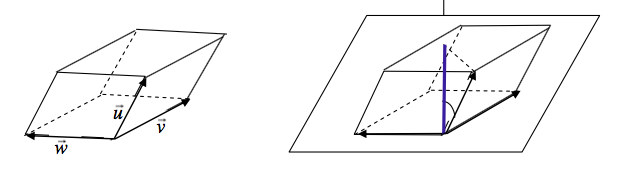
\includegraphics[height=3cm]{volum}
%\end{figure}


\end{document}